

\begin{frame}{Linear Algebra on GPUs}

 \begin{block}{Consider Something Simple}
  \begin{itemize}
   \item $x \leftarrow y$, $x,y \in \mathbb{R}^N$, distinct
   \item Usually a simple for-loop, memory-bandwidth limited
  \end{itemize}
 \end{block}

 \begin{center}
  \only<1>{ 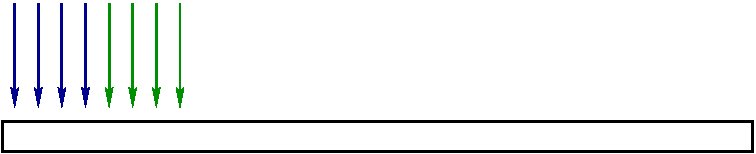
\includegraphics[width=0.8\textwidth]{figures/vec-gpu-scalar-1} }
  \only<2>{ 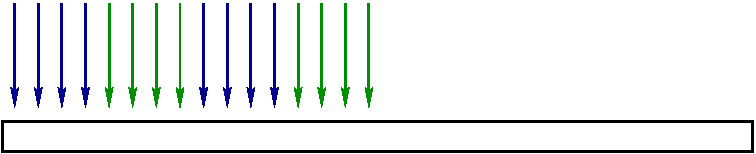
\includegraphics[width=0.8\textwidth]{figures/vec-gpu-scalar-2} }
  \only<3>{ 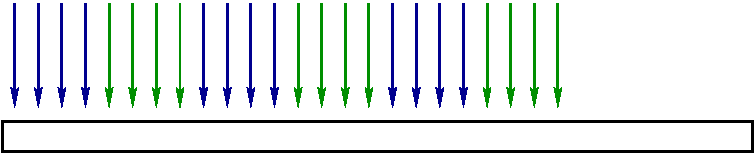
\includegraphics[width=0.8\textwidth]{figures/vec-gpu-scalar-3} }
  \only<4>{ 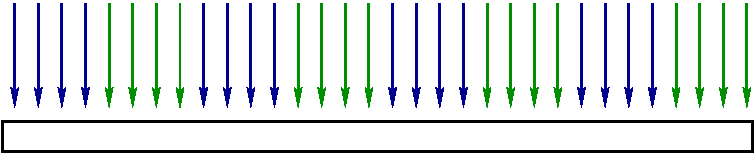
\includegraphics[width=0.8\textwidth]{figures/vec-gpu-scalar-full} }

  \only<5>{ 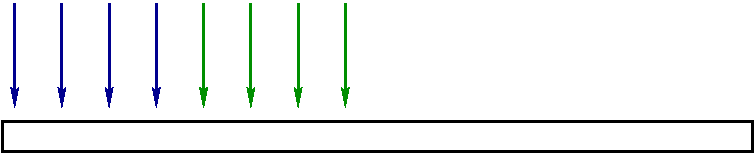
\includegraphics[width=0.8\textwidth]{figures/vec-gpu-vec-1} }
  \only<6>{ 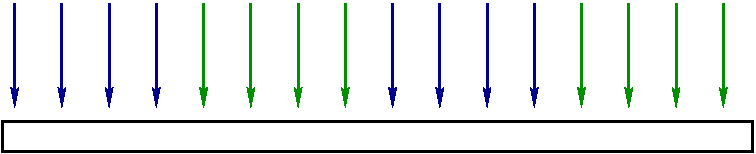
\includegraphics[width=0.8\textwidth]{figures/vec-gpu-vec-full} }
  
  \only<7>{ 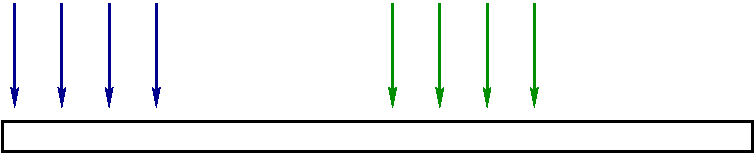
\includegraphics[width=0.8\textwidth]{figures/vec-cpu-vec-1} }
  \only<8>{ 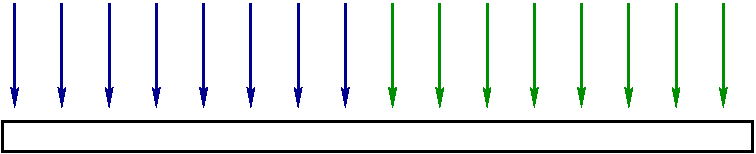
\includegraphics[width=0.8\textwidth]{figures/vec-cpu-vec-full} }
 \end{center}

\end{frame}



\begin{frame}{Linear Algebra on GPUs}

 \begin{block}{Consider Something Simple}
  \begin{itemize}
   \item $x \leftarrow y$, $x,y \in \mathbb{R}^N$, distinct
   \item Usually a simple for-loop, memory-bandwidth limited
  \end{itemize}
 \end{block}

 \begin{block}{Parameters}
  \begin{itemize}
   \item Data Types: \lstinline|double|, \lstinline|double2|, etc.
   \item Blocking: Small segments vs. large blocks
   \item Thread sizes: threads per group, number of thread groups
  \end{itemize}
  \vspace*{-0.3cm}
 \end{block}

\end{frame}


\begin{frame}{Linear Algebra on GPUs}

 \begin{block}{OpenCL Benchmarking Baseline}
  \begin{itemize}
   \item \lstinline|double|
   \item small segments
   \item 128 threads per work group
   \item 128 work groups
  \end{itemize}
 \end{block}

 \begin{block}{Results (GB/sec)} 
  \begin{center}
  \begin{tabular}{|l|c|c|c|c|}
   \hline
   Name           & \footnotesize\lstinline|double|, small, 128x128 & \footnotesize Best & \footnotesize \lstinline|double2|, large, 32x240 \\
   \hline
   NVIDIA GTX 285   & 101 & 134 & 134 \\
   NVIDIA GTX 580   & 150 & 166 & 123 \\
   AMD HD 7970      & 161 & 249 & 140 \\
   INTEL E5-2670 x2 &  32 &  79 &  18 \\
   INTEL Xeon Phi   &  32 &  95 &  21  \\
   \hline
  \end{tabular}
  \end{center}
 \end{block}

\end{frame}






\begin{frame}{Vector Addition Benchmarks}
  \begin{center}
   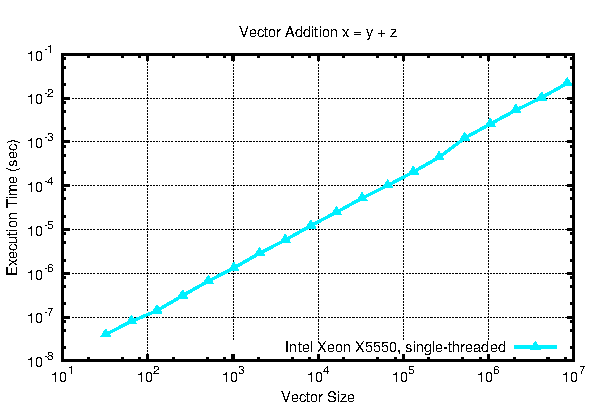
\includegraphics[width=0.95\textwidth]{figures/vector-timings-1}
  \end{center}
\end{frame}

\begin{frame}{Vector Addition Benchmarks}
  \begin{center}
   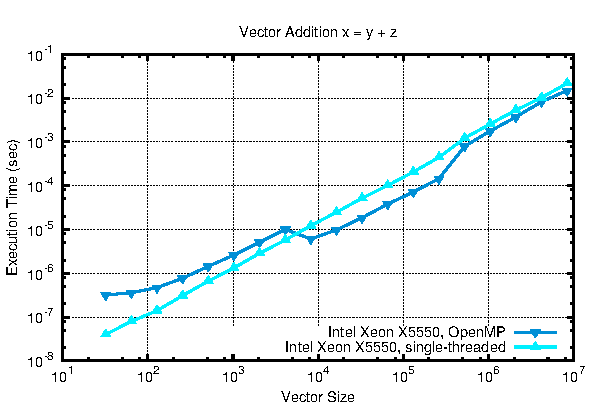
\includegraphics[width=0.95\textwidth]{figures/vector-timings-2}
  \end{center}
\end{frame}

\begin{frame}{Vector Addition Benchmarks}
  \begin{center}
   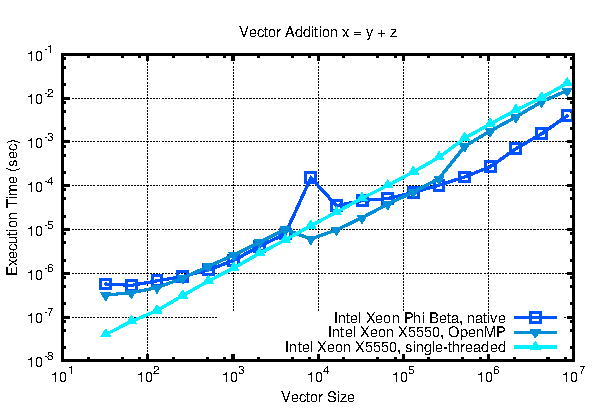
\includegraphics[width=0.95\textwidth]{figures/vector-timings-3}
  \end{center}
\end{frame}

\begin{frame}{Vector Addition Benchmarks}
  \begin{center}
   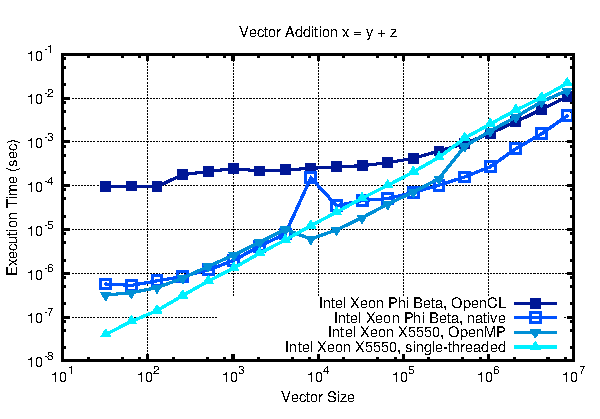
\includegraphics[width=0.95\textwidth]{figures/vector-timings-4}
  \end{center}
\end{frame}

\begin{frame}{Vector Addition Benchmarks}
  \begin{center}
   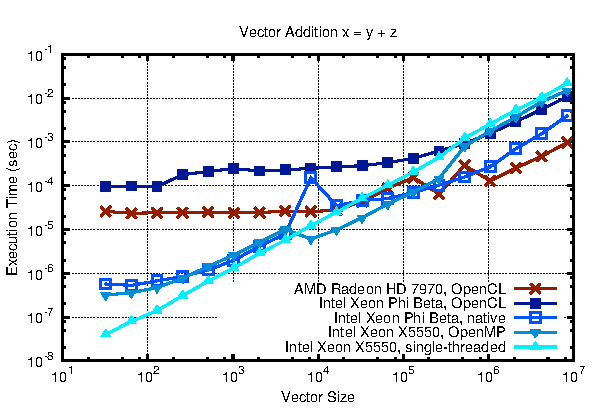
\includegraphics[width=0.95\textwidth]{figures/vector-timings-5}
  \end{center}
\end{frame}

\begin{frame}{Vector Addition Benchmarks}
  \begin{center}
   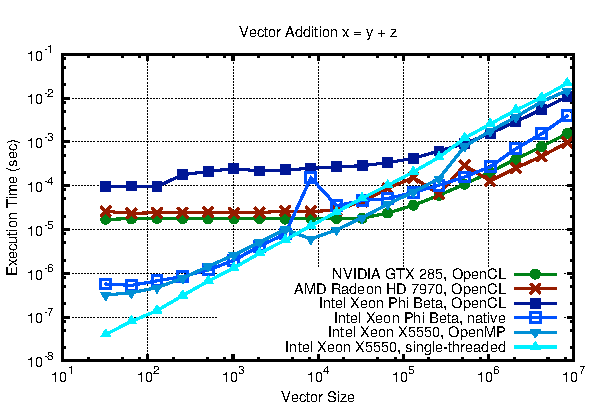
\includegraphics[width=0.95\textwidth]{figures/vector-timings-6}
  \end{center}
\end{frame}

\begin{frame}{Vector Addition Benchmarks}
  \begin{center}
   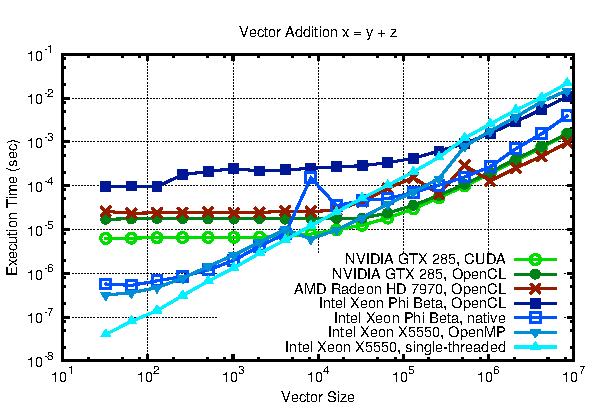
\includegraphics[width=0.95\textwidth]{figures/vector-timings-7}
  \end{center}
\end{frame}



\begin{frame}{Matrix-Matrix Multiplication}
 \begin{block}{Parameter Space Explosion}
  \begin{itemize}
   \item Global Block Sizes
   \item Shared Mem Block Sizes
   \item Thread-Private Block Sizes
   \item Loop Unrolling
  \end{itemize}
 \end{block}
 
   \begin{center}
   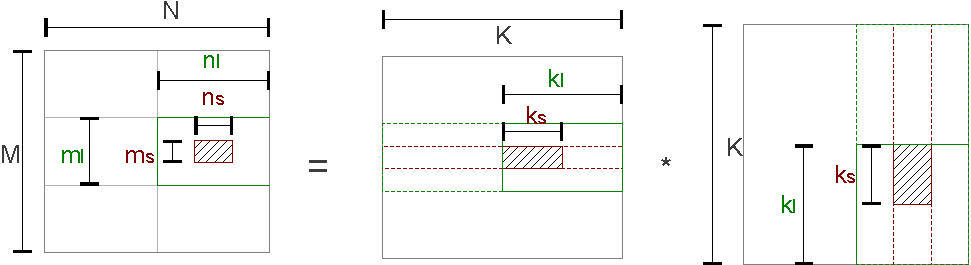
\includegraphics[width=0.95\textwidth]{figures/MatrixMatrixProduct}
  \end{center}

\end{frame}



\begin{frame}{Matrix-Matrix Multiplication}
  \begin{center}
   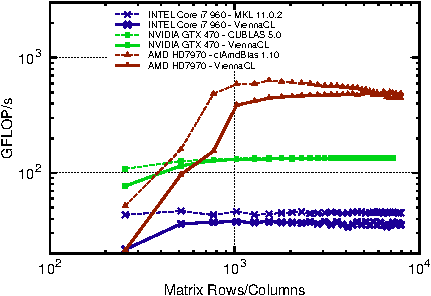
\includegraphics[width=0.95\textwidth]{figures/dgemm}
  \end{center}
\end{frame}

\begin{frame}{Matrix-Matrix Multiplication}
  \begin{center}
   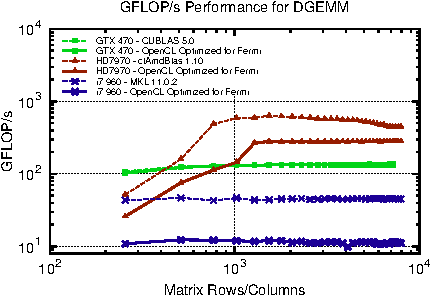
\includegraphics[width=0.95\textwidth]{figures/cross-benchmark-3-double}
  \end{center}
\end{frame}

